\section{Modelamiento}
En esta sección se presenta el procedimiento de la creación, que consta de tres etapas relevantes, y selección del modelo para lograr los objetivos del trabajo y finalmente presentar el Sistema de Predicción de la Deserción Escolar (SPDE).

\subsection{Selección de Variables de Entrada}
Nuestra muestra de estudio contiene alrededor de 90 variables de diferentes índoles. El hecho de utilizar la totalidad de variables hará que el algoritmo de aprendizaje automatizado se demore demasiado. Dada esta limitante, escogeremos las variables más relevantes utilizando un algoritmo de aprendizaje automatizado llamado bosques aleatorios, lo que hace es calcular la importancia de las variables, es decir, las que tienen mayor poder de discriminación. Aparte de este método existen varios más como por ejemplo la varianza de las variables\footnote{Entre más varianza, mayor poder de discriminación}, otro método se señala como \textit{KBest}, que lo que hace es permutar las variables hasta encontrar la mejor combinación. El bosque aleatorio hace algo parecido a esto último.

En la Figura~\ref{fig:impo-total1} podemos observar las variables que poseen mayor poder de discriminación. Es decir, las variables de entrada seleccionadas son las siguientes:\\
\begin{itemize}
\item Sobre-Edad del Alumno
\item Percentil de Promedio General en el curso y grado
\item Percentil de la Asistencia en el curso y grado
\item Escolaridad básica de los padres
\item Grupo socioeconómico de la manzana del establecimiento y hogar
\item Convivencia promedio en el establecimiento(OIC)
\item Pago de la matrícula anula y costo mensual
\item Información de la selección de alumnos en la admisión del establecimiento
\item Autoestima y motivación promedio en el establecimiento(OIC)
\item Participación promedio en el establecimiento(OIC)
\item Escolaridad superior de los padres
\end{itemize}
\begin{figure}[H]
  \centering
    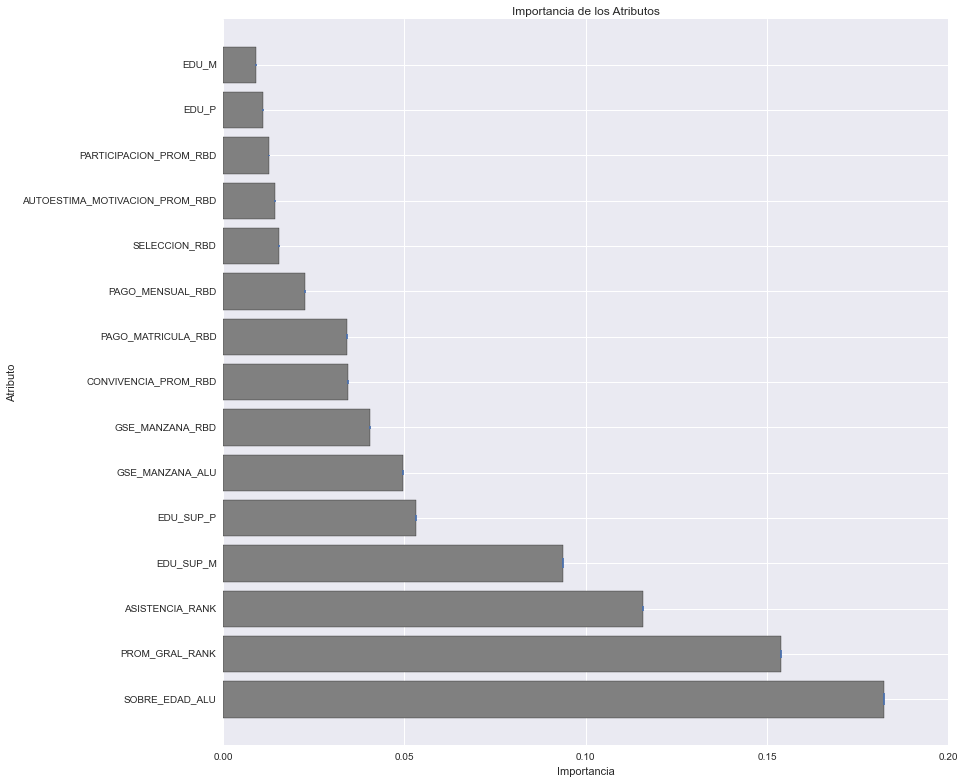
\includegraphics[trim=0cm 0cm 0cm 0cm,scale=0.4]{Figuras/7AnalisisResultado/impo-total.png}
      \caption{Importancia de las variables de entrada del modelo de predicción utilizando Bosques Aleatorios con todas las variables disponibles}
    \label{fig:impo-total1}
\end{figure}
\subsection{Selección de Algoritmo de Aprendizaje Automatizado}
Para poder seleccionar el algoritmo de aprendizaje automatizado que se utilizará en el modelo de predicción, es necesario realizar una comparación en base a una medida comparable entre las diferentes técnicas y aproximaciones para lograr las predicciones. Lo que se desea predecir es la deserción escolar al próximo año y esta información se contiene en la variable $DESERTA\_ALU$, donde a través de variables de entradas se desea predecir el valor de la variable de salida $DESERTA\_ALU$. Esta variable objetivo toma valor 1 cuando el alumno deserta, y valor 0 cuando no lo hace, por tanto, definiremos que cuando $DESERTA\_ALU = 1$, entonces se define como la clase desertora y $DESERTA\_ALU = 0$ como la clase no desertora.

El procedimiento para seleccionar el algoritmo de aprendizaje automatizado será el siguiente:
\begin{enumerate}
\item Selección de algoritmos de aprendizaje automatizados viables obteniendo una lista $a_1, a_2, a_3, ..., a_n$ de algoritmos a probar: Para poder seleccionar los algoritmos, primero se llevó a cabo una revisión exhaustiva de la documentación de la librería de aprendizaje automatizado utilizada\footnote{http://scikit-learn.org/stable/documentation.html} y se seleccionaron en base a lo estudiado de la teoría. La lista de algoritmos a evaluar se puede ver en la Tabla~\ref{tab:lista-algo}.

Para poder seleccionar los algoritmos se debe tomar en cuenta las características de la muestra de estudio. En base a la exploración realizada en la sección anterior, encontramos que el conjunto de datos está fuertemente desbalanceado, es decir, tenemos aproximadamente de 260.000 alumno existen solamente 7.000 alumnos desertores. Esto claramente presenta un desafío para algunos métodos tradicionales. Para poder superar este desafío existen varias opciones que incluye sobre-muestrear\footnote{En la literatura existe un método de sobre-muestra muy utilizado llamado SMOTE(\textit{Synthetic Minority Over-sampling Technique})} la clase que pertenece a la minoría hasta obtener el balance total de las clases. El problema de esto es que se tendrían aproximadamente 500.000 casos para entrenar el modelo, lo que haría sumamente alta la complejidad del algoritmo de aprendizaje automatizado. Hay que mencionar también que la librería, en algunos métodos, tiene implementada cierta funcionalidad que permite entregarle un peso relativo a cada clase de forma automatizada, pero esto no ocurre para todos los algoritmos, por tanto, si bien es una opción viable, no podríamos evaluar algoritmos que son prometedores. Finalmente, el único método que se ajusta a todos, e incluso podemos reducir notablemente el tiempo computacional de los métodos no-lineales con complejidad muy alta, es muestrear aleatoriamente la clase que pertenece a la mayoría. Utilizando este método obtendríamos aproximadamente 15.000 alumnos, donde la mitad son desertores y la otra mitad son alumnos no desertores muestreados.

Finalmente, debido al procedimiento señalado anteriormente, podemos utilizar todos los algoritmos de la Tabla~\ref{tab:lista-algo} para hacer las pruebas de los modelos de predicción.

\cuadro{6SolucionPropuesta/lista-algo}

\item Prueba de cada uno de los modelos de predicción utilizando el algoritmo de aprendizaje automatizado y buscando sus hiper-parámetros lo más cercano posible al óptimo. \\ \hfill
Para poder escoger el algoritmo que se utilizará en el modelo de predicción, se desarrolló un \textit{script} en Python utilizando diferentes librerías donde se evalúa automáticamente cada modelo y se realiza la optimización de hiper-parámetros de cada uno de estos, lo que se puede ver en el Anexo~\ref{an:cselect}.

A continuación se detalla el procedimiento automático que realiza el \textit{script}:\\
\begin{enumerate}
\item Creación de una muestra aleatoria de la clase de alumnos no desertores con el fin de dejarla del mismo tamaño que la clase desertora, es decir, aproximadamente una muestra de 7.500 alumnos no desertores de 250.000 no desertores \footnote{La clase se define como el objetivo que se busca predecir, es decir, en este caso tenemos dos clases: El alumno desertará(1) o el alumno no desertará(0).}.
\item División estratificada\footnote{Esto quiere decir que se tomaron en cuenta la cantidad de desertores y no desertores para tomar una muestra que contenga la misma proporción para así no generar sesgos en el entrenamiento.} en un \textbf{conjunto de datos de entrenamiento externo} que contiene el 70\% de los datos y un \textbf{conjunto de prueba externo} que contiene el 30\%.
\\ \hfill
Ahora para cada modelo $a_i$ con parámetros $p_i$ seleccionado:
    \begin{enumerate}
    \item División aleatoria del conjunto de prueba externo en 10 subconjuntos de igual tamaño llamados \textbf{conjuntos de prueba y entrenamiento internos}\footnote{Esto se señala en la literatura como \textit{k-fold validation} con $k = 10$, y es muy útil para obtener una medida de desempeño con baja varianza y realista.}.
    \item Se toma el primer subconjunto para el entrenamiento para crear un modelo de predicción utilizando el algoritmo $a_i$ y los parámetros del modelos $p_i$, luego se evalúa el desempeño del algoritmo utilizando los 9 subconjuntos restantes.
    \item Se seleccionan, en base al procedimiento de la búsqueda aleatoria de parámetros, los mejores parámetros con los que se logra el mejor desempeño automáticamente. Para esto se define una grilla de 10 valores basada en una distribución logarítmica y distribución uniforme de enteros.\footnote{En la teoría se señala que este método entrega resultados buenos, cercanos al óptimo, pero nunca se llega a este puesto que al probar 10 de 50 conjuntos de parámetros de forma aleatoria no podemos se puede asegurar un óptimo. Si se haría una búsqueda exhaustiva de los parámetros, es decir, evaluar todos los valores posibles dentro del conjunto de parámetros dados podemos asegurar esto, pero lamentablemente la capacidad computacional sería altísima resultando impracticable con los recursos actuales utilizados para el trabajo.} .
    \end{enumerate}
Se repite el procedimiento anterior para cada subconjunto existente para cada algoritmo $a_i$ y sus parámetros cercanos al óptimo $p_i$, es decir, se obtienen 10 mediciones del desempeño del modelo de predicción $a_i$ y se obtiene su desviación estándar, junto con el tiempo de entrenamiento utilizado\footnote{Este tiempo cuenta el procedimiento total, no el tiempo de entrenamiento real, como el procedimiento es una suma de varios entrenamiento, podemos utilizarlo como aproximación al tiempo real.}. Este procedimiento en particular se puede observar en la Figura~\ref{fig:metosel}.
\end{enumerate}
\item Se ordenan los resultados obtenidos de cada $a_i$ algoritmo en base a la medición del desempeño de cada uno, se genera un \textit{ranking} de los algoritmos probados y se selecciona al mejor en base a este, donde la posición menor en el \textit{ranking} es mejor.
\item Finalmente, ya seleccionado de forma automatizada el algoritmo de predicción que se ajusta mejor a los datos sin ningún tipo de sesgos gracias al complejo procedimiento de validación cruzada utilizada, se entrena el modelo utilizando dicho algoritmo con sus parámetros cercanos al óptimo con el conjunto de entrenamiento externo sin realizar subdivisiones de este, es decir, con el 30\% de los datos disponibles. De este nuevo modelo de predicción se obtiene su medición de desempeño y así, con este mismo modelo, se evalúa el desempeño del resto de los datos que corresponde al conjunto de datos de prueba externo para compararlo con la medición del desempeño de la muestra de prueba, es decir, el error de generalización $E_{gen}$ es la diferencia entre la medición del desempeño en el conjunto de entrenamiento externo y la medición del desempeño en el conjunto de prueba externo.
\end{enumerate}

\begin{figure}[H]
  \centering
    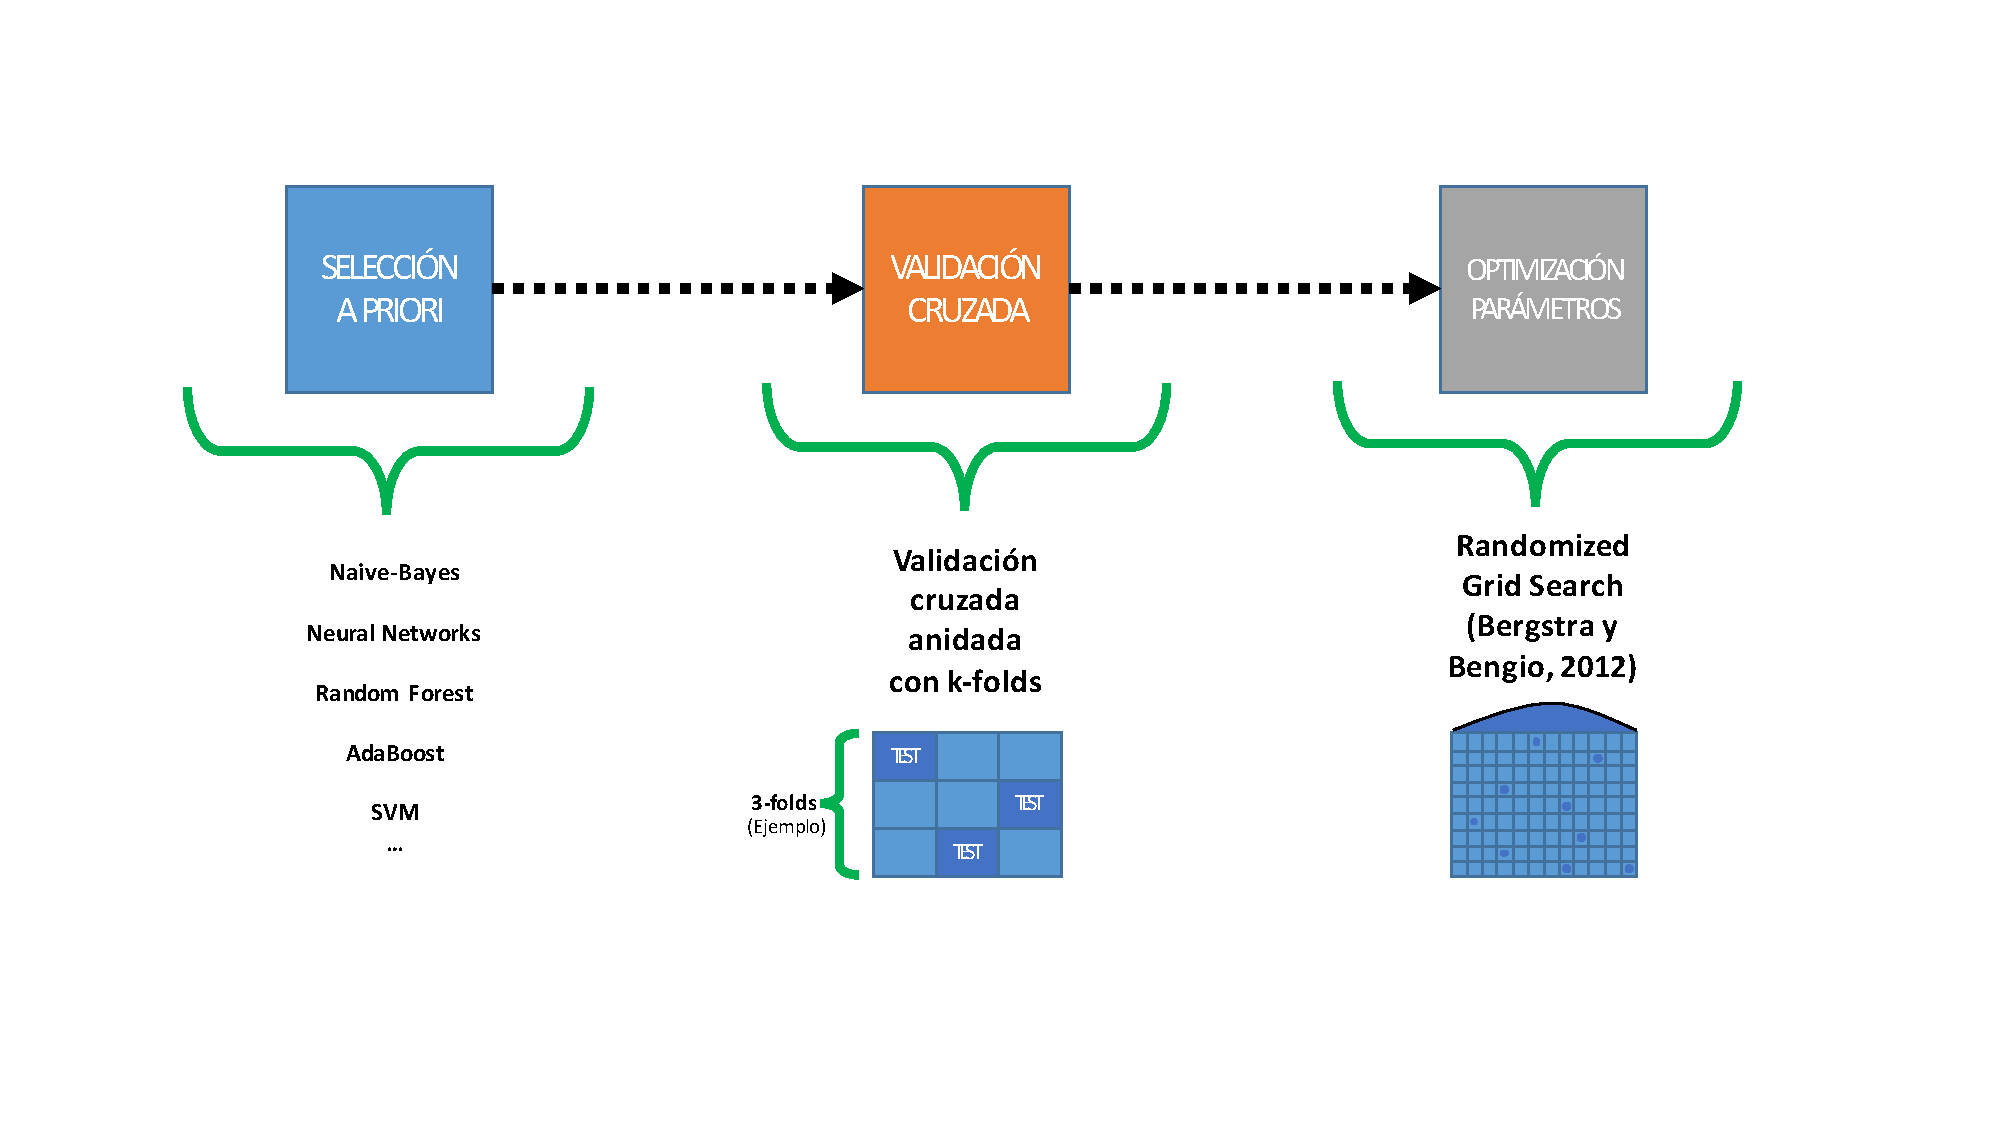
\includegraphics[trim=0cm 5cm 0cm 0cm,,scale=0.5]{Figuras/6SolucionPropuesta/metosel.pdf}
      \caption{Procedimiento de selección del algoritmo de aprendizaje automatizado}
    \label{fig:metosel}
\end{figure}

Al utilizar el \textit{script} que se puede ver en el Anexo~, se genera la Tabla~\ref{tab:smodelr} donde se muestra un \textit{ranking} de los 9 mejores algoritmos ordenados del mejor (posición nº1 en el \textit{ranking}) al peor (posición nº9). El mejor algoritmo de aprendizaje automatizado es AdaBoost con exhaustividad del 89,71\% en promedio\footnote{Recordemos que esto se obtuvo realizando 10 mediciones utilizando diferentes conjuntos de entrenamiento y prueba(validación cruzada interna)} y una desviación estándar de 0,98\% en un tiempo de 67 segundos. Analizando los demás algoritmos, podemos ver que las diferencias son mínimas entre el \textit{ranking} 2 y 3, por tanto podríamos ser indiferentes entre AdaBoost, \textit{Random Forest} (Bosques Aleatorios) y SVM con Kernel Polinomial, pero si comparamos los tiempos es posible notar que el tiempo del SVM con Kernel Polinomial son 488 segundos, mientras que los demás tienen un promedio de 60 segundos. Esto es importante si se piensa que el modelo de predicción debe alojar gran cantidad de datos, por esta razón se descarta el algoritmo en el \textit{ranking} 3 y se opta por escoger el algoritmo AdaBoost.

\cuadro{6SolucionPropuesta/smodelr}

Finalmente, los parámetros del modelo seleccionado se pueden observar en la Tabla~\ref{tab:params}. El primero se llama \textit{Learning Rate}, que muestra cuánto contribuye cada algoritmo al resultado de la clasificación y la cantidad de estimadores (algoritmos). Recordemos que AdaBoost no es un algoritmo, sino más bien un meta-algoritmo, pues lo que busca es mejorar la estimación agregando más estimadores, que en este caso, son árboles de decisión. Es decir, se van agregando árboles de decisiones enfocándose en mejorar la clasificación de alumnos desertores.

\cuadro{6SolucionPropuesta/params}

\subsection{Creación del Modelo de Predicción}
Una vez seleccionado el mejor algoritmo de aprendizaje automatizado, una última prueba involucra al poder de generalización del modelo de predicción creado. Esto es muy importante realizarlo debido a que puede que, a través del procedimiento de selección del modelo, se generen sesgos en el entrenamiento del modelo de predicción. Esto sucede ya que al escoger aquel modelo que entrega el mejor desempeño en base a la predicción del conjunto de entrenamiento se puede estar incluyendo un par de parámetros y algoritmo de aprendizaje automatizado que se ajustan muy bien a los datos entregados, pero no así a los datos que el modelo no conoce.\footnote{Esto también se hace referencia como al sobre-ajuste(\textit{overfitting}) de un modelo de predicción.}. Debido a que nuestro procedimiento de selección de modelo se realizó solamente utilizando la porción interna de la división de los conjuntos de datos de la validación cruzada, es necesario probar el poder de generalización del modelo de predicción, para lo que se utilizará la validación externa. En el Cuadro~\ref{tab:smodelr} podemos ver el resultado de la clasificación del modelo de predicción en el conjunto de prueba externo.

\cuadro{6SolucionPropuesta/confu}

Si comparamos lo obtenido con el resultado del Cuadro~\ref{tab:confu} observamos que se obtuvo un 88\% de exhaustividad de la clase de desertores. Al calcular el error de generalización\footnote{Esto nosotros lo definimos como el desempeño del conjunto de entrenamiento menos el desempeño del conjunto de prueba.} se ve que es menor a 0, lo que nos señala que el modelo de predicción tiene un buen poder de generalización y no sufre de un sesgo importante.

Dicho lo anterior, podemos concluir que el modelo de predicción posee un poder de predicción del 89\% para predecir casos futuros. Esto claramente se podría mejorar si se logra obtener mayor volumen de datos, y además, una mayor capacidad computacional para entrenar el modelo de predicción con estos.

\subsection{Presentación del Sistema de Predicción de la Deserción Escolar}
Ahora, una vez creado el modelo de predicción, tenemos que lograr que este modelo tenga la capacidad para funcionar con otros sistemas, específicamente con un sistema o plataforma que sea capaz de visualizar los datos que predice el modelo de predicción. Para lograr esto, lo que se debe hacer es utilizar algún método que permita darle capacidad de interacción al modelo de predicción. Nosotros optamos por incrustar una API\footnote{Una API(\textit{Application Programming Interface}) es un conjunto de funciones de programación que permiten interactuar de forma sencilla con algún sistema o programa. En otras palabras es una capa de abstracción para comunicarse con otros componentes} para realizar futuras comunicaciones en tiempo real con el modelo de predicción.

Para esto, se trabajó con una librería de Python llamada Flask que tiene la capacidad para recibir peticiones HTTP\footnote{Protocolo usado en transacciones web para visualizar y enviar información desde un navegador.} y enviar datos mediante el mismo protocolo. Además se utilizó la librería Joblib que permite hacer persistente al modelo de predicción dando la posibilidad de guardar el modelo en un archivo para después ser cargado cuando sea necesario.

En el API se implementó el método 'predict', que permite enviar información de un alumno al modelo a través de una página web para después entregar la información de predicción a la persona que hizo la petición. Otro método útil para el modelo, que en este caso no se implementó, es el de 'train' que se utiliza para entrenar con nuevos casos al modelo de forma agregada, es decir, se van acumulando los casos pasados del alumno, pues si a futuro cambian los patrones de la deserción el modelo no quede obsoleto.\footnote{Esto se decidió no implementar, puesto que el algoritmo utilizado en este trabajo para entrenar al modelo no permite esto. Esto en la literatura se refiere al procedimiento de \textit{partial-fit}.}.

El método 'predict' que se implementó recibe las variables de entrada a través de una solicitud HTTP POST\footnote{Esto es una solicitud HTTP de envío de información hacia el servidor HTTP que maneja la API.} de los parámetros siguientes:
\begin{enumerate}
\item Características personales del Alumno
    \begin{itemize}
    \item MRUN
    \item SOBRE_EDAD_ALU
    \item PROM_GRAL_RANK
    \item ASISTENCIA_RANK
    \end{itemize}
\item Características del contexto familiar y convivencia del Alumno
    \begin{itemize}
    \item EDU_SUP_P
    \item EDU_SUP_M
    \item ING_HOGAR
    \item GSE_MANZANA_ALU
    \end{itemize}
\item Características del contexto familiar y convivencia del Alumno
    \begin{itemize}
    \item SELECCION_RBD
    \item GSE_MANZANA_RBD
    \end{itemize}
\end{enumerate}

La respuesta a esta solicitud HTTP POST entrega dos parámetros en formato JSON\footnote{JavaScript Object Notation(JSON) es un formato de datos ligeros para el intercambio fácil de información entre diferentes sistemas.En conjunto con el formato de datos XML, se utiliza mucho para salida de información(\textit{endpoints}) de las API.}:
\begin{itemize}
\item MRUN
\item DESERTA_ALU
\end{itemize}

Un conjunto de variables seleccionadas del modelo original fue excluido solamente para efectos de demostración de la capa de abstracción. El código utilizado para implementar esto se puede revisar en el Anexo~\ref{an:cspde}. De ahora en adelante, el modelo de predicción se señala como el Sistema de Predicción de la Deserción Escolar (SPDE).

Para mostrar el funcionamiento del SPDE utilizaremos dos casos de prueba que pueden ser vistos en la Tabla~\ref{tab:test-spde}. Al enviar una solicitud HTTP POST mediante un navegador de internet a la dirección URL donde se encuentra funcionando el servidor del API\footnote{Para esta demostración se utiliza \url{http://localhost:8000/predict?param1=value2&param2=value2...}}.
\cuadro{6SolucionPropuesta/testSistema}

Se obtiene a continuación la siguiente respuesta de parte del SPDE:
\begin{enumerate}
\item  \textbf{Alumno de Prueba 1} \\ \hfill
\begin{minted}[frame=single,
               framesep=3mm,
               linenos=true,
               xleftmargin=21pt,
               tabsize=4]{js}
{     
    "MRUN": 12543245,
    "DESERTA_ALU" : 0
}
\end{minted}
\item  \textbf{Alumno de Prueba 2} \\ \hfill
\begin{minted}[frame=single,
               framesep=3mm,
               linenos=true,
               xleftmargin=21pt,
               tabsize=4]{js}
{     
    "MRUN": 3653265,
    "DESERTA_ALU" : 1
}
\end{minted}
\end{enumerate}

Interpretando estos datos, el SPDE nos señala que el Alumno de Prueba 2, desertará en el presente año (2013), y por tanto, no registrará matrícula en el año 2014, mientras que del Alumno de Prueba 1 se señala que sí se mantendrá en el sistema regular.

Finalmente, ya tenemos definido como funciona el SPDE y su capa de abstracción mostrando que la implementación del SPDE es sumamente sencilla. Para poder aprovechar el SPDE, es necesario incorporar un sistema de información que almacene y vaya registrando la información futura de los alumnos a estudiar con la finalidad de mostrar visualizaciones útiles para la toma de decisiones. En la Figura~\ref{fig:SPDE} se muestra el caso hipotético del diseño de cómo se debiese incorporar una plataforma de visualización al SPDE. La plataforma de visualización es un complemento del sistema para que cualquier persona con un computador pueda utilizar y aprovechar el SPDE, sin necesidad de tener conocimiento directo de este. Igualmente, como se puede observar en la Figura~\ref{fig:SPDE}, se sugiere que el sistema de visualización tenga las siguientes funcionalidades:
\begin{enumerate}
\item Base de datos persistente \\ \hfill
La plataforma debe funcionar con una base de datos persistente que contenga todos los alumnos registrados que serán sometidos a evaluación con sus diferentes características, esto para apoyar la visualización. Esta base de datos, más precisamente, debe contener la información que será evaluada por el modelo y los índices importantes como el establecimiento al que asiste el alumno, su identificación única(MRUN), coordenadas, etc..
\item Visualizaciones
    \begin{itemize}
    \item Lista de desertores en un establecimiento especifico(Nivel Alumno) \\ \hfill
    La lista de desertores en un establecimiento es una visualización útil para entregarle herramientas de toma de decisiones al mismo establecimiento afectado, es decir, estos van a poder hacer un seguimiento, detectar grados donde aumenta la deserción basada en su contexto habitual. Con esto, será posible, debido a la ventaja de tener individualizados a los alumnos, hacer un seguimiento al alumno con problemas establecimiento planes de acción para revertir la situación.
    \item Comunas con sus respectivas tasa de deserción pronosticadas en un mapa interactivo(Nivel Comunal) \\ \hfill
    Esta visualización muestra el mapa del Gran Santiago con las tasas de deserción pronosticadas de cada comuna mostrándose en diferentes colores dependiendo de la cantidad de desviaciones estándar que tiene cada comuna en base al promedio. Esta herramienta es útil para el MINEDUC, debido a que pueden monitorear la deserción a nivel agregado, y como la mayoría de los establecimientos son municipalizados, pueden pedir más información detallada a esta que finalmente son los que sostienen a los establecimientos.
    \item Lista de los establecimientos con mayor tasa de deserción en un mapa interactivo(Nivel Establecimiento) \\ \hfill
    La lista de establecimientos muestra los establecimientos con mayores tasas de deserción o los establecimientos donde su tasa de deserción difiere mucho en base al promedio. Esto es muy útil para que las municipalidades puedan monitorear el estado de la deserción y tomar medidas en establecimientos en especifico, que básicamente es su interés.
    \end{itemize}
\item Formulario para envío de alumnos a evaluar \\ \hfill
La plataforma debe tener la capacidad para que a través de alguna especie de formulario se puede enviar la información a la API. Esta información correspondería a las variables de entrada del sistemas más el índice del alumno para mantener la identificación.
\item Formulario para agregar alumnos a los datos de entrenamiento del modelo\footnote{Esto es opcional, puesto que depende de la compatibilidad con el algoritmo de aprendizaje automatizado, en el caso de este trabajo el algoritmo no es compatible. Esto se deja solamente para señalar que sí es posible hacer un modelo que vaya evolucionando sin necesitar algoritmos genéticos. En la literatura esto se señala como \textit{partial-fit}.} \\ \hfill
Esto es para entrenar el modelo con los alumnos nuevos que ya han sido sometidos a prueba(y cuando se obtiene verdaderamente su información en base a la permanencia o no del alumno en el sistema de educación regular)
\end{enumerate}
%Todo esto se puede ver resumido en la Figura~\ref{fig:Sistema}, donde se muestra el SPDE(Llamado Motor de Predicción) y la plataforma de visualización sugerida anteriormente.
\begin{figure}[H]
  \centering
    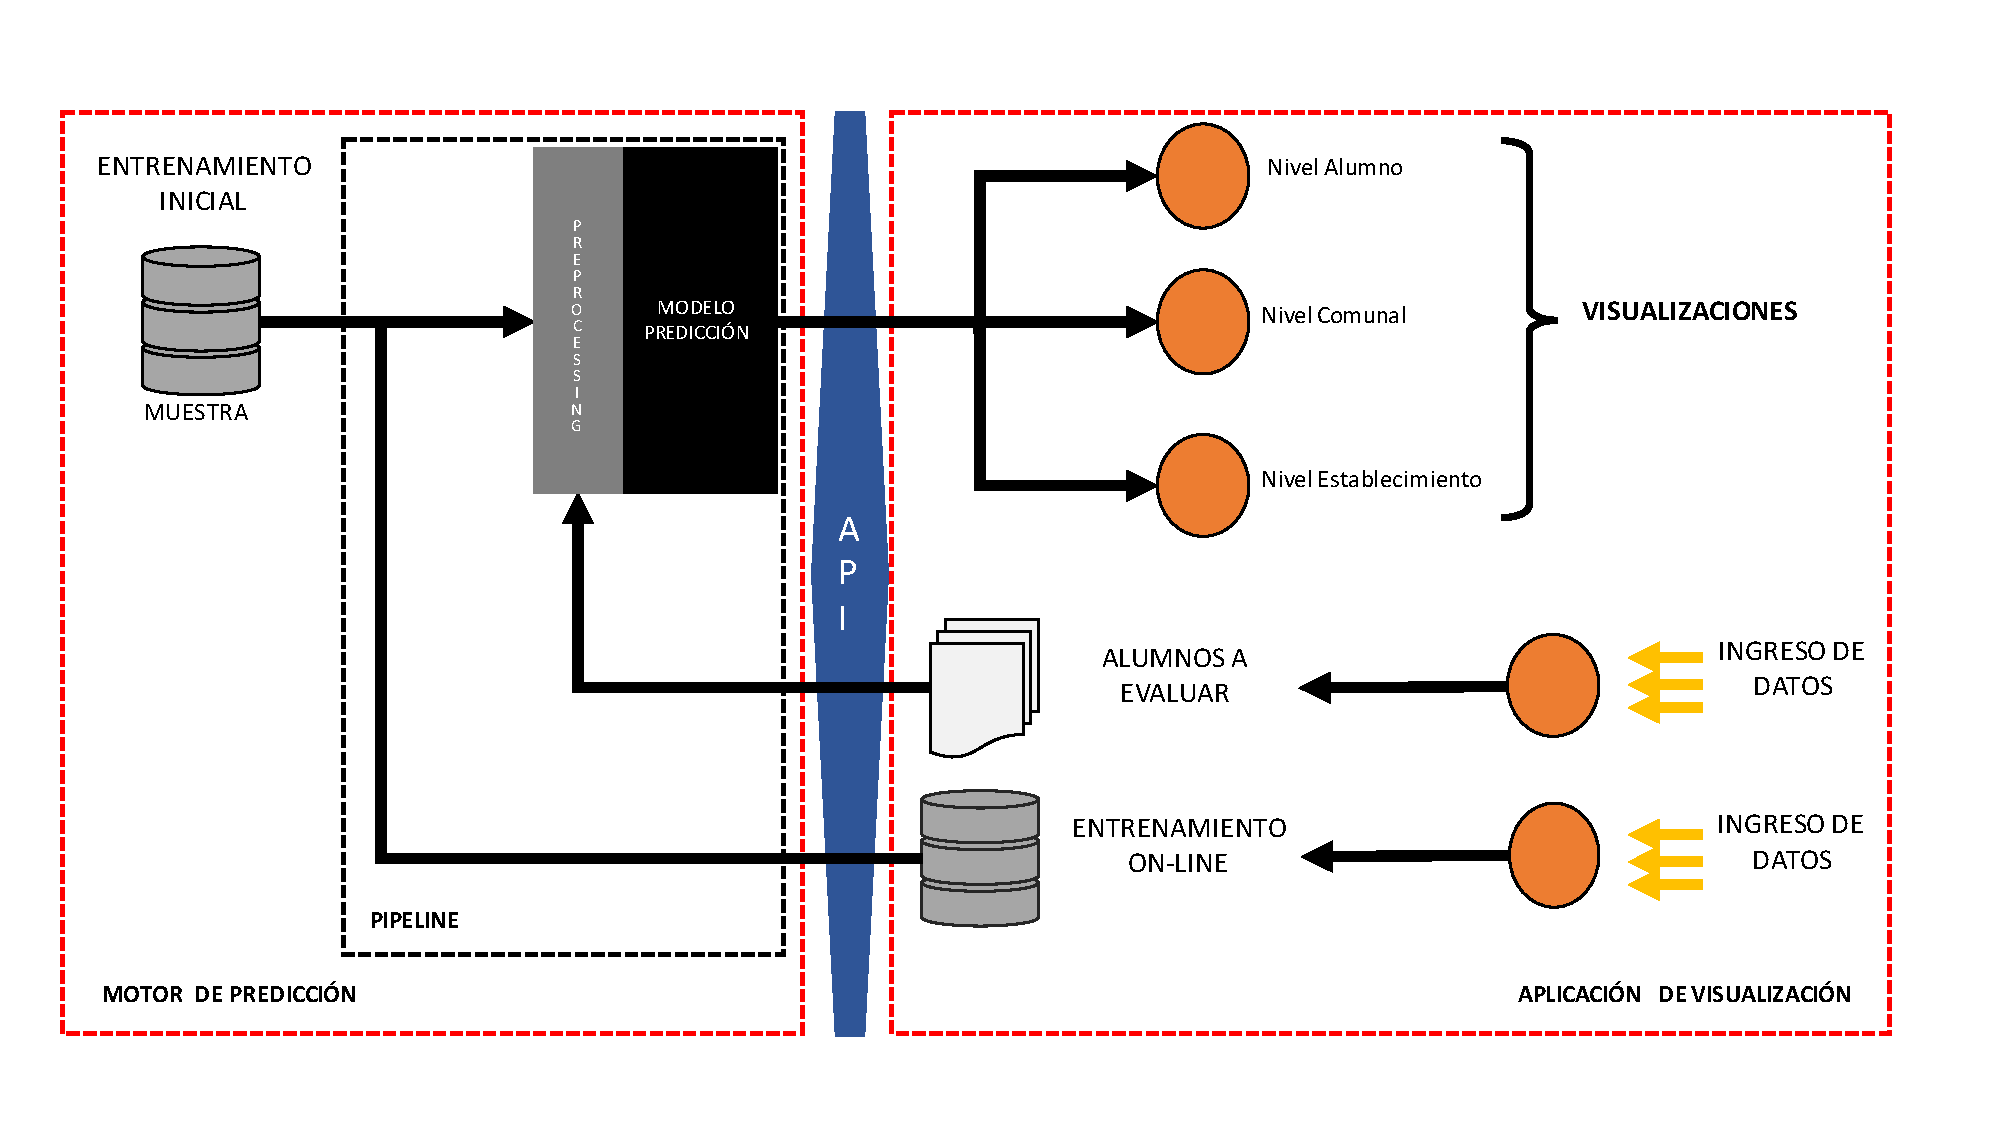
\includegraphics[trim=0cm 0cm 0cm 0cm,scale=0.45]{Figuras/6SolucionPropuesta/Sistema.pdf}
      \caption{Diseño del SPDE con la plataforma de visualización sugerida para la interacción.}
    \label{fig:SPDE}
\end{figure}

